\documentclass{acm_proc_article-sp}

\begin{document}

\title{Mining Jazz: An Experience Report}
\numberofauthors{1} 
\author{
Thanh H.D. Nguyen, Adrian Schr\"oter, Daniela Damian\\
	   \affaddr{Software Engineering Global interAction Lab (SEGAL)}\\
       \affaddr{Department of Computer Science}\\
       \affaddr{University of Victoria}\\
       \affaddr{Victoria, British Columbia, Canada}\\
       \email{\{duythanh, schadr, danielad\}@uvic.ca}
}
\maketitle

% Abstract
\begin{abstract}
Integrated collaborative software engineering tools such as IBM
Jazz\texttrademark provide researchers opportunities to access a 
vast amount of information that reflects the real development activities 
of software teams. With all of the artifacts stored in one place and 
linked together, researchers can gain valuable insights about the 
teams' collaborative activities. We report on our experience in mining the Jazz 
development team repository to study collaboration in sofware develpment. In
particular we explain the different options and constraints we had
during our efforts to mine the Jazz repository. In addition, we show
some results we obtained by studying communication practices in the Jazz
project team to demonstrate our research with data obtained from the mining
process.
%We think our experience is applicable to any research data mining project not just only on Jazz but for any other collaborative software engineering tools.
\end{abstract} 

% Formality
% A category with the (minimum) three required fields
%\category{H.4}{Information Systems Applications}{Miscellaneous}
%A category including the fourth, optional field follows...
%\category{D.2.8}{Software Engineering}{Metrics}[complexity measures,
%performance measures]

%\terms{Delphi theory}

%\keywords{ACM proceedings, \LaTeX, text tagging} % NOT required for Proceedings


% Introduction
\section{Introduction}
Accessing research data in Software Engineering is very difficult. Regardless of
the project methodology, the high cost of labour and developers' stressful
workload are always big challenges that researchers face in their effort ot
access developers' working environment. On the other hand, software developers
usually utilize digital media to coordinate their work. This media is 
usually archived and thus can be used for research as it provides valuable
insights into the developers' activities. For example, the bugzilla bug
tracking database of several open-source development teams have been studied in
the past~\cite{bettenburg:2007:tr}. So did developer mailing lists, emails~\cite{Bird:2006:MSR}, or even IRC chat~\cite{Cataldo:2006:CSCW}.


However, this media are usually not connected to each other. It is very difficult
for researchers to link artifacts such as a bug on bugzilla and a post on the
developer mailing list to make them useful for research. Fortunately, the advent
of integrated end-to-end collaboration development environtments such as IBM Jazz~\cite{IBM:2008:url} provides research with opportunities to explore the development activities without having to take away developers' valuable working hours or manually connecting different artifacts from different media. In
this paper, we are describing our experience in data mining the IBM Jazz team
collaboration. In the next section, we present our conceptualization of doing
research via artifacts as well as challenges we encountered. Then we explain the
importance of the IBM Jazz development environtment to research. In Section 4, we
explain the diffent options and contraints we have during the mining process.
Section 5 outlines the three design principles we learned from building the data
mining tool. And finally, in Section 6, we provide some results of a research
project we did based on the data we mined in Jazz.




% Motivation
\section{Research via artifacts}
Our research methodology applied and extended the growing knowledge of mining
software repositories~\cite{msr08}. Figure~\ref{fig:Framework} illustrates the
process of mining and leveraging software artifacts for research as we
conceptualize it. The goal is to study different kinds of \emph{Software
Development Activities}, such as planning, designing, implementing, or testing a
product. With the use of \emph{integrated development environments}, the
activities are recorded. In highly integrated collaboration development
environments such as Jazz, the record of development activities are kept in the
form of different artifacts such as plans, work items, or source code changes. We
opted to infer knowledge from the created artifacts, because gathering data
directly from the developers, through surveys or interviews, are often highly
invasive and very time consuming for researchers.


 \begin{figure}[t]
	\begin{center}
	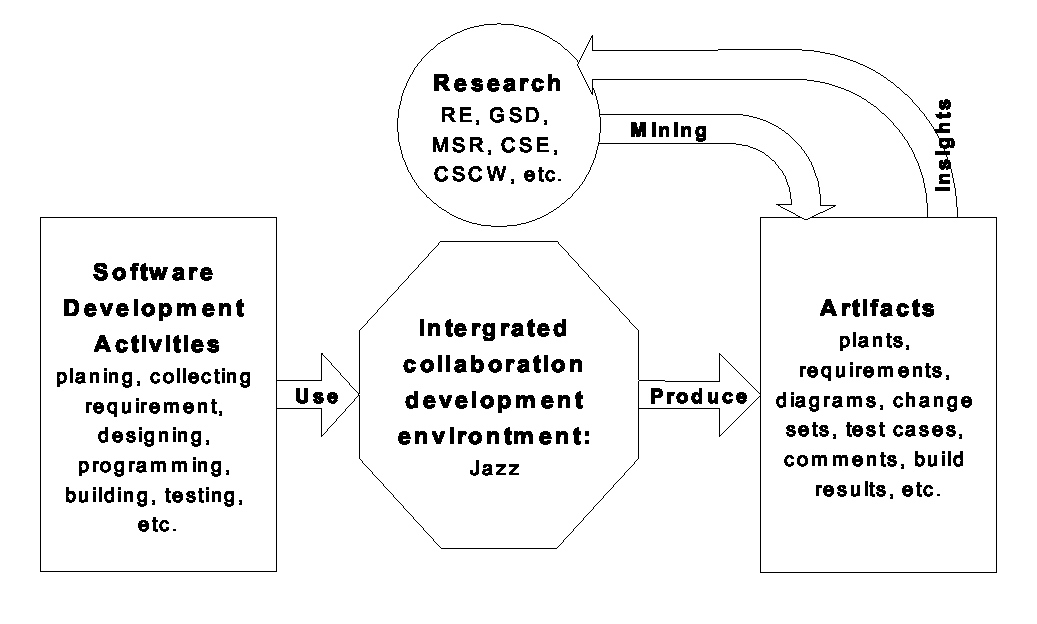
\includegraphics[width=.99\columnwidth]{./Figures/Figure01Framework}
	\caption{The research via artifacts process}
	\label{fig:Framework}
	\end{center}
\end{figure}

The mining and studying of development artiacts has its own specific
challenges as well. Two main challenges are:
\begin{enumerate}
\item The complexity of the data mining task.
\item The validity of insights obtained through the artifacts.
\end{enumerate}
The first challenge is a technical one. It raise questions such as ''How to
get access to the data?''. The data mining process can be very complex and
sometimes impossible. As we will explain in sbsequent sections, it requires
careful planing and implementation. The second challenge is on the research level. By
doing research via artifacts, we have to make inferences about the software
development activities through the artifacts it produces. This makes it hard to
interpret the result. The main questions center around ''How to interpret the
artifacts?'' and ''Is our interpretation valid?''.

The importance of these challenges depends on the point of view. For the
development team the first challenge is more relevant because extracting data
from a repository might crash it or delay the development process in other ways.
Whereas the second challenge is of more relevance to research. Researchers are
always interested in new findings, growing, or validating the body of knowledge.
After leveraging the two point of views, the big question that we are trying to
answer is: How to build a Jazz data mining tool that minimizes the effort of
both the development team and the researchers, and maximizes the validity of our
study? Before we discuss our approach to addressing this question, we briefly
describe the IBM Jazz project in the next section and explain why we
decided to build the data mining tool.


% Why Jazz
\section{Why Jazz}
Jazz~\cite{Cheng:2003:ACMQueue,frost:2007:IEEESoftware} is a development
environment that integrates programming, communication, and project management.
The main goal of Jazz is to bring collaboration support for all of the software
development activities such as planning, building, testing, and reporting. For
developer, this means that they can communicate and coordinate their work through
the very same tools they use to develop code. To achieve this, Jazz provides a
central repository for all tools supporting the development process such as a planning
wiki, a work item tracking system, a report component, and a build system.

At the time of our study, Jazz consisted of three major
components~\cite{IBM:2008:url}:
\begin{itemize}
\item The Jazz repository. 
\item The Rational Team Concert (RTC) client.
\item The dashboard, a web user interface.
\end{itemize}
The \emph{Jazz repository} stores all artifacts available to the two clients. 
Examples for such artifacts are work items, comments, and build results. 
The \emph{RTC client} is the main development client. 
It is built upon the Eclipse platform and allows developers to control their work spaces, to perform version control functions, and to request builds. 
The \emph{web user interface} allows developers to access most of the non-coding related artifacts, such as work items, iteration plans, and reports. 

For researchers, Jazz provides an easy way to extract valuable research data. Due
to the tight integration of the different components, links of artifacts to
related software development activities already exists. For example, a comment
is linked to tasks, also called work items, and source code changes in the form
of change sets are attached to these work items. This is a major advancement to
other systems that used their own heuristics to link software
artifacts~\cite{cubranic:2003:icse}.

%So if a build is red, we can find all of the communication around the build and, subsequently, construct the communication network associate with the red build.

%In the next section we explore the different options to extract Jazz data and the constraints we face during the process.



% Information to research
\section{Options and Constraints}
The Jazz repository gave us several choices on how to extract data from it: via the dataware house report, via the RTC client API, via the server API, and via the back-end database. Each of these choices comes with its own constraints. These constraints can be summarized in three categories: (1) the \emph{effort} needed, (2) the \emph{logistical overhead} in terms of travel or non legal permissions, and (3) the \emph{legal} issues such as guaranteeing the privacy of developers. In  addition to these constraints the four choices provided by the Jazz repository differ in the system level they are deployed at.
 
\begin{table}[h]
\begin{center}
{\small
\begin{tabular}{|c|c|c|c|}
\hline \textbf{Option} & \textbf{Effort} & \textbf{Logistic} & \textbf{Legal} 	\\
\hline                
Report		& Hard 		& Easy	 	& Easy	\\ 
\hline
Client API	& Medium-Hard	& Medium	& Easy-Medium	\\ 
\hline
Server API	& Medium-Hard	& Medium-Hard	& Medium	\\ 
\hline
Database	& Easy		& Medium	& Hard	\\ 
\hline
\end{tabular}
}

\end{center}
\caption{Our simple risk analysis based the available options and the constraints}
\label{tab:OptionsVsConstraints}
\end{table}%

\begin{description}
\item[Report]
The report component in Jazz caches performance statistics of the Jazz repository
and provides mechanisms to assess this information via the Jazz Dashboard. We
could build a report that queries the data from the Jazz team server.

The draw back in terms of effort following this option is that we need to learn
how to set up the report and obtain the data from the given data warehouse. Note
that the report component had changed since then. In term of effort, this option
became easier now. Logistically, this is the easiest option because the report
can be deployed and obtained online. It is also the easiest option in term of
legal requirement because all of the information in the dataware house are
supposed to be public. \item[Client API] Using the RTC client API we can write a
plug-in to access the data via the RTC client. This plug-in can query  the data
that is available to the client and serialize the result. We can then import the
result into a relational database.

The effort we need to spend in developing a plug-in using the client API lies in
learning it. Although we are familiar with Java and Eclipse technologies, the
APIs were constantly changed. More importantly, we are also restricted to the queries
that are available to the client. We have to search the client code to find
suitable queries and work around their restrictions. In terms of logistic, the
development can be done off-site. The deployment have to be done on-site but it
is not difficult because the query can be run inside a standard developer set up.
Using the client API does not require a lot of legal advise because most data
that is available through the client is available to the public.

\item[Server API] Another option to query the data is bypassing all the client
APIs and access the Jazz repository itself. This way we are still restricted
by the repository API but not by the client API. Note that these APIs are not formally
defined yet at the time of writing this article.

Since we can bypass the client API, this option would take less effort on the
programming. But it requires deep understanding of what the repository can
provide. The learning process would have take as much effort as the client API
option. In term of logistic, we would be able to run it on-site and it is harder
to debug off-site because it can not be run from a nornal client. It may require
working on-site with the repository team. Legally, this option can be tricky
because we could get information that are not normally available to the public.
\item[Database Backend] If we are allowed, we can also acquire a copy of the
backend database of the Jazz repository.

This option would be the least effort in term of programming. However, it would
be very difficult, in term of legal requirement, to warranty privacy and
intellectual property of the compant. Even if we are allow to, we would require
to manage the task of getting the large data set and extracting the useful
information from the raw data.

\end{description}

Table ~\ref{tab:OptionsVsConstraints} shows the simple risk analysis we did based on the options available and the constraints. We decided to obtain the data via the RTC client API. This option seem to have the average of medium risk. In term of effort, it is very time consuming but we have the resources to manage. For us, the logistic and legal requirement are more important and they are manageable on this option.


% Methodology
\section{Design principles}
The main requirement for our tool besides being able to extract all data is to
not cause any problem in the development cycle of the team, such as causing to
much load on their repository while extracting the data. We implemented these
requirements in a program that was developed in several iterations.

\paragraph{Iterative} 
At the beginning of developing our mining tool, we evaluates the data that was
available through the RTC client API. We found that the API did not support the
extraction of all the data so we proceeded with an iterative development that was
oriented at the different kind of data accessible through the API at a time.
Similar to iterations in an Agile process, we extended the extraction capability
of the tool one by one via adding data query set. At the end of each iteration,
we asked our research contact at IBM to extract more data with the updated tool.
This had the advantage that we received additional feedback about API usage from
our IBM research contact.

\paragraph{Minimally Invasive} 
The data quantity we want to extract can cause a high load on the repository and
thus disrupt the development process, each time we extract the data.
% After several iteration, our query set started to put very high load on the
% main repository which prevented developers access to it.
We avoided causing such high repository load by updating the existing data
instead of extracting all data every time we run the program. This had the
advantage in case we finished a new query we did not need to extract all the data
we extracted earlier again.

\paragraph{Separation}
In order to keep the additional load minimal on the repository we tried to remove
redundancies in the queries as well as avoid the queries to load data that has
already been extracted. At the beginning, some of our queries depended on each
other or we could not avoid loading already extracted data. For example, if we
wanted to fetch the new comments on work items, we had to fetch the work items
themselves although they had not changed since the last extraction. This
introduced additional load on the repository. We removed all unnecessary
dependencies among queries and tried to minimize loading data that has already
been extracted.

% We think those decisions were important to the success of the project and may
% be useful for future research.



% Expected Result
\section{Communication delay project}
This project ~\cite{Nguyen:2008:ICGSE} used data we mined as described in this
paper and we describe it as an illustration of our
design principles and conducting research using software development artifacts.

There were two main objectives of this project: (1) to examine if the Jazz team
experience communication and task completion delay due to the large geographic
distance between the teams and (2) gain insights about communication patterns of
the entire project team. For the first objective, we conceptualized communication
delay as the difference between comments on work items and task completion delay
by the resolution time of a work item. Thus, we had to query all work items from
the Jazz repository. With the information on work items we addressed our second
objective by constructing and examining a project-wide communication-based
social network that connecting developers that commented on the same work items.

\begin{figure}[t]
	\begin{center}
	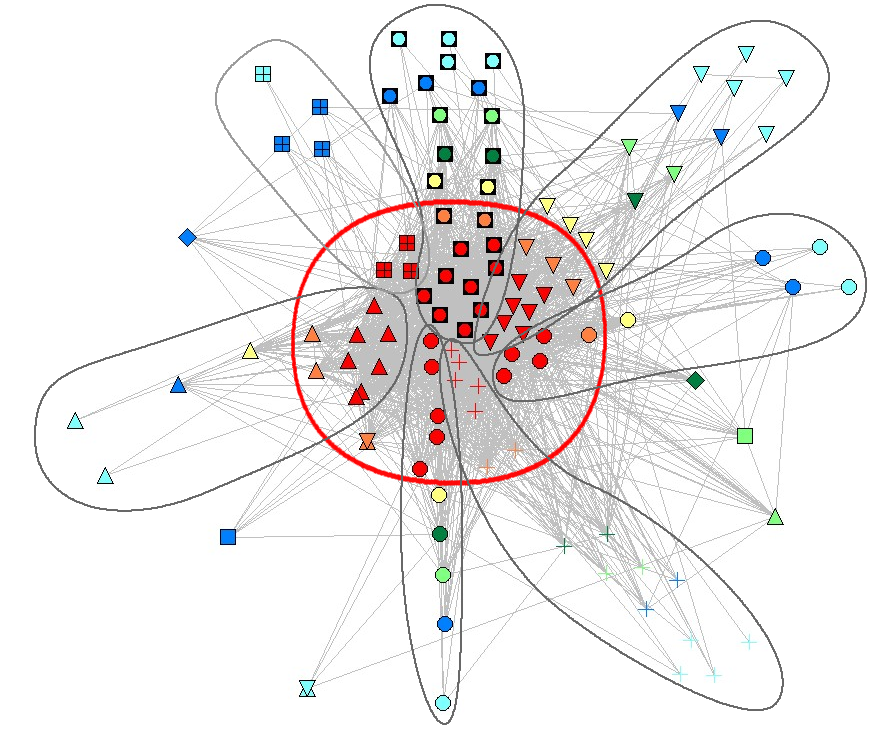
\includegraphics[width=.99\columnwidth]{./Figures/Figure03SocialNetwork}
	\caption{The communication based social network of the Jazz development team}
	\label{fig:SocialNetwork}
	\end{center}
\end{figure}

Following an iterative process, we first designed a query for a teams' hierarchy.
Subsequently, we wrote a query to retrieve the members of each team. In
the next iteration we designed the query to retrieve all work items. This query
induced a high load on the repository due to the large amount of data that was
contained in all work items. During the early versions of Jazz we encountered
client and server side failures cause by our query. To minimize the additional
load generated from re-running a crashed query, our tool stores a cache of the
queried data which does not need to be extracted during the re-run. When it is
resumed, the query picks up from where it left. We were able to extend the tool
and extract the data within the first six months of our project.

With the information from the work items, our analysis suggests that
the Jazz team did not experience as much delay as reported in previous
literatures~\cite{Battin:2001tb,Herbsleb:2003oo}. We hypothesize that this is due
to the new integrated development support provided by Jazz as well as advances
in software practices used by the Jazz distributed team.

Using this data we also constructed the project-wide social network based on communication as shown in Figure~\ref{fig:SocialNetwork}. The shape of the nodes (and the flower-like petals) indicate the developers' geographical location. The color of the nodes indicate how active each developers is in the overall network from most active (red) to least active (light blue). The red circle emphasizes the active core members of the project.

% Conclusion
\section{Conlusion}
Mining the Jazz repository has been a challenging journey. In
this paper we shared our experiences and the lessons we learned during the
process: iterative, minimal invasive, and separation. We think that the design principles we presented here
are applicable to any research via artifact projects regardless of the repository
behind it.

For us, the Jazz data continue to be a very valuable source of information. The
artifacts in Jazz hold valuable insights about both the social and technical
aspects of the Jazz team's development process. Obtaining the communication and
coordination data in one place creates numeorous of possibilities for researchers
to look at various aspects of intricate software development activies all
together, and which were very hard to do with research methods other than
repository mining. With the release of Jazz and the adoption of technology by
many of the Eclipse based products from IBM, we think that mining the Jazz
repositories will bring more and more benifits to research.

% Acknowledgments
%ACKNOWLEDGMENTS are optional
\section{Acknowledgments}
We want to thank all members of the IBM Jazz project who helped us, particularly
Harold Ossher, Li-Te Cheng of IBM TJ Watson, and Jean-Michel Lemieux of IBM Ottawa Lab. Many thanks to the members of the SEGAL lab. Funding was provided by  NSERC and IBM Jazz Technology
Fellowship Award. 

IBM and Jazz are trademarks of IBM Corporation in the US, other
countries, or both.


% Appendix
% %APPENDICES are optional
%\balancecolumns
\appendix
%Appendix A
\section{Headings in Appendices}
The rules about hierarchical headings discussed above for
the body of the article are different in the appendices.
In the \textbf{appendix} environment, the command
\textbf{section} is used to
indicate the start of each Appendix, with alphabetic order
designation (i.e. the first is A, the second B, etc.) and
a title (if you include one).  So, if you need
hierarchical structure
\textit{within} an Appendix, start with \textbf{subsection} as the
highest level. Here is an outline of the body of this
document in Appendix-appropriate form:
\subsection{Introduction}
\subsection{The Body of the Paper}
\subsubsection{Type Changes and  Special Characters}
\subsubsection{Math Equations}
\paragraph{Inline (In-text) Equations}
\paragraph{Display Equations}
\subsubsection{Citations}
\subsubsection{Tables}
\subsubsection{Figures}
\subsubsection{Theorem-like Constructs}
\subsubsection*{A Caveat for the \TeX\ Expert}
\subsection{Conclusions}
\subsection{Acknowledgments}
\subsection{Additional Authors}
This section is inserted by \LaTeX; you do not insert it.
You just add the names and information in the
\texttt{{\char'134}additionalauthors} command at the start
of the document.
\subsection{References}
Generated by bibtex from your ~.bib file.  Run latex,
then bibtex, then latex twice (to resolve references)
to create the ~.bbl file.  Insert that ~.bbl file into
the .tex source file and comment out
the command \texttt{{\char'134}thebibliography}.
% This next section command marks the start of
% Appendix B, and does not continue the present hierarchy
\section{More Help for the Hardy}
The acm\_proc\_article-sp document class file itself is chock-full of succinct
and helpful comments.  If you consider yourself a moderately
experienced to expert user of \LaTeX, you may find reading
it useful but please remember not to change it.
\balancecolumns
% That's all folks!



%
% The following two commands are all you need in the
% initial runs of your .tex file to
% produce the bibliography for the citations in your paper.
\bibliographystyle{abbrv}
\bibliography{2008-iReCoSE}  % sigproc.bib is the name of the Bibliography in this case
% You must have a proper ".bib" file
%  and remember to run:
% latex bibtex latex latex
% to resolve all references
%
% ACM needs 'a single self-contained file'!
%
\end{document}